\mode*

\section{Behållare}

\subsection{Listor}

\begin{frame}[fragile]
  \mintinline[fontsize=\huge,escapeinside=||]{python}{var = [ item0, |$\dotsc$|, itemN ]}
\end{frame}

\begin{frame}[fragile]
  \begin{example}
    \begin{minted}{python}
names = ["Adam", "Bertil", "Cesar"]
print(names[0])
print(names[2])
    \end{minted}
  \end{example}
\end{frame}

\begin{frame}
  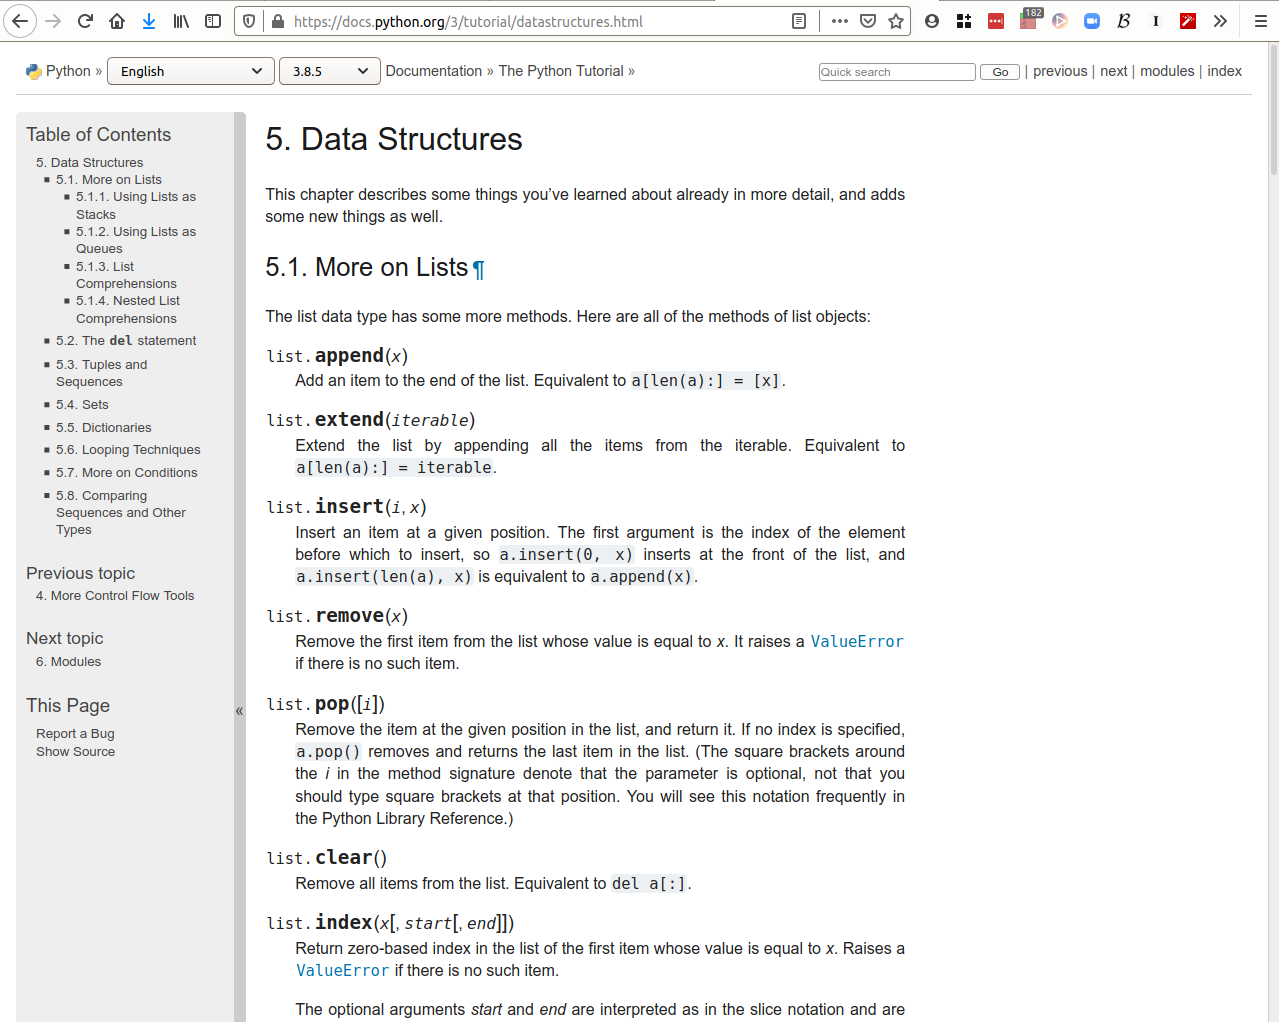
\includegraphics[width=\columnwidth]{figs/docs-lists.png}
\end{frame}

\begin{frame}[fragile]
  \begin{example}[extend\textunderscore{}lists.py]
    \inputminted{python}{examples/extend_lists.py}
  \end{example}
\end{frame}

\begin{frame}[fragile]
  \begin{example}[Aritmetiska \emph{hel}talsföljder]
    \begin{minted}{python}
print(range(10))
print(range(0, 10))
print(range(1, 10, 2))
    \end{minted}
  \end{example}
\end{frame}


\begin{frame}[fragile]
  \mintinline[fontsize=\huge]{python}{var = [ f(x) for x in lst ]}
\end{frame}

\begin{frame}[fragile]
  \begin{example}[List comprehensions]
    \begin{minted}{python}
squares = [ x**2 for x in range(10) ]
    \end{minted}
  \end{example}
\end{frame}


\subsection{Stackar och köer}

\begin{frame}[fragile]
  \begin{example}[pile.py]
    \inputminted{python}{examples/pile.py}
  \end{example}
\end{frame}

\begin{frame}[fragile]
  \begin{example}[queue.py]
    \inputminted{python}{examples/queue.py}
  \end{example}
\end{frame}

\begin{frame}
  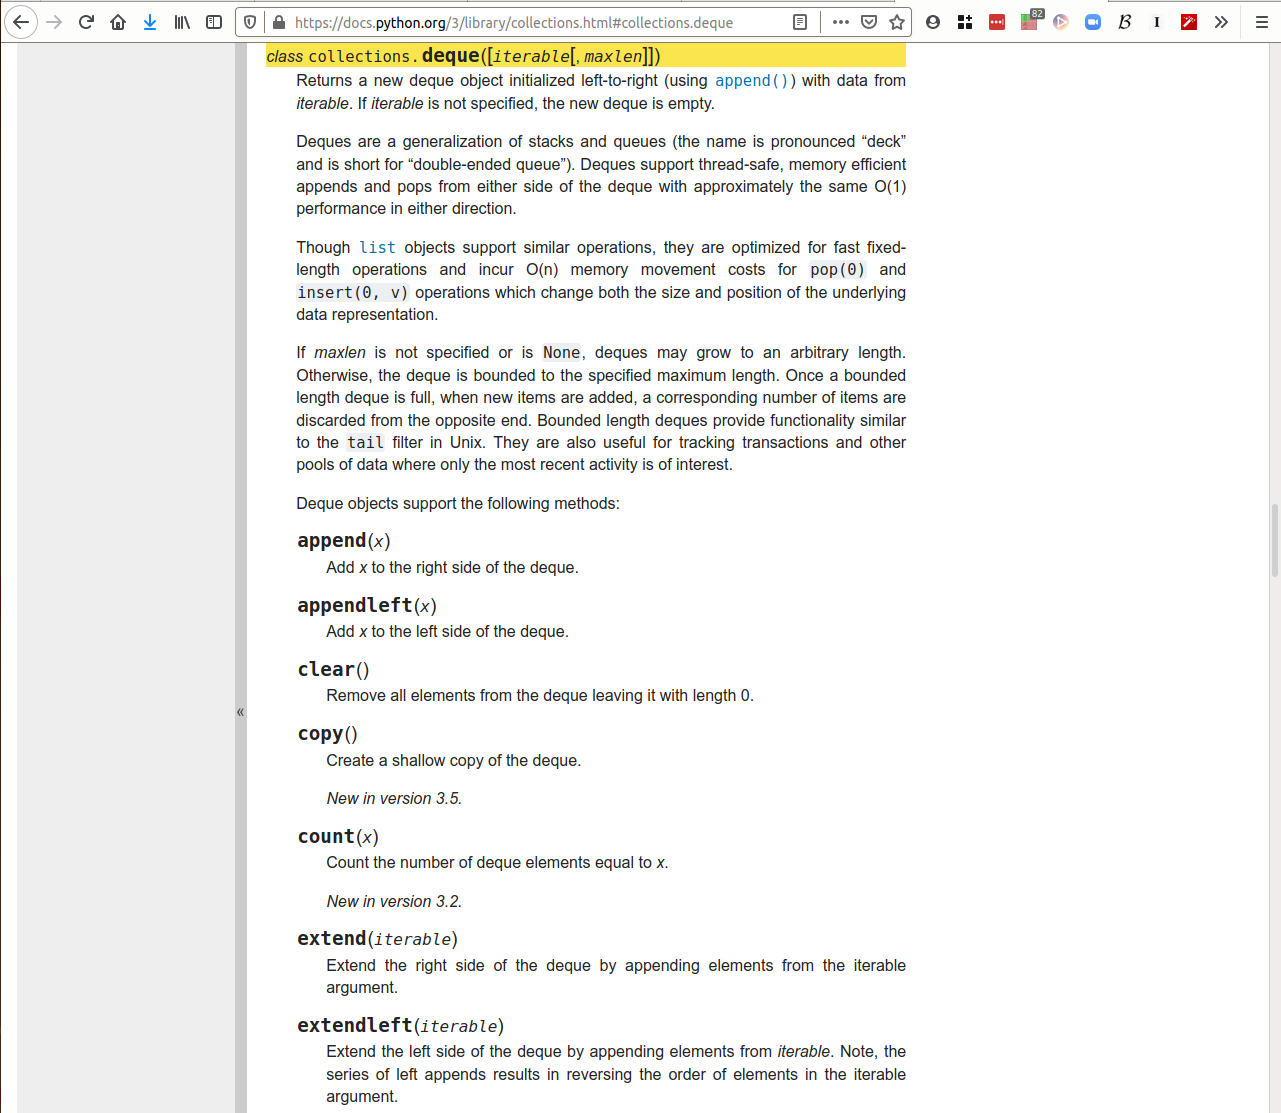
\includegraphics[width=\columnwidth]{figs/docs-deque.png}
\end{frame}


\subsection{Mängder}

\begin{frame}[fragile]
  \begin{example}[sets.py]
    \inputminted{python}{examples/sets.py}
  \end{example}
\end{frame}


\subsection{Uppslagslistor}

\begin{frame}
  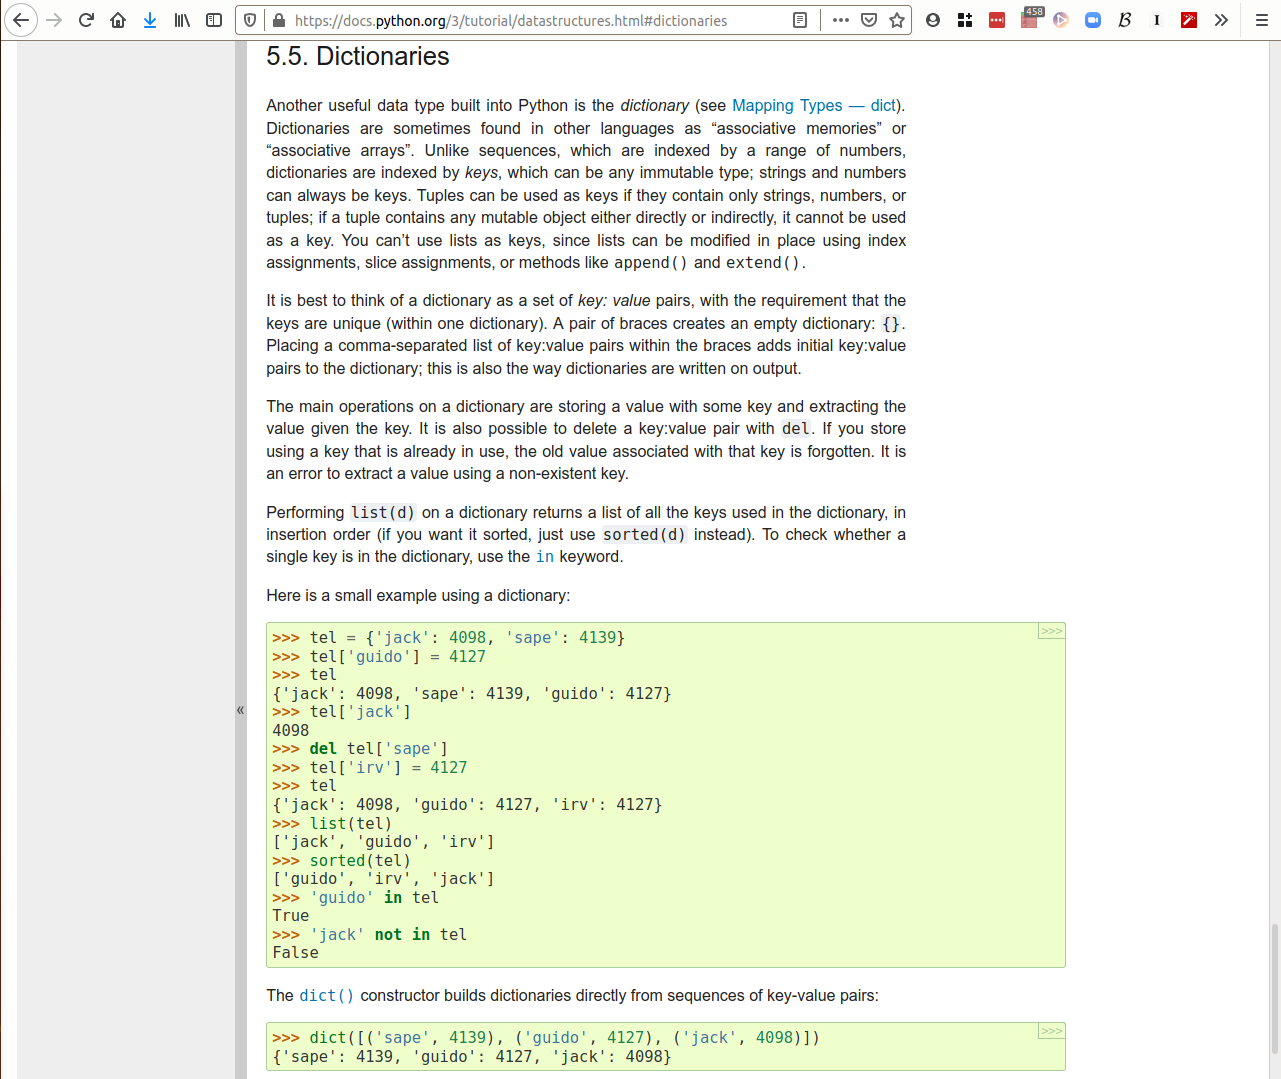
\includegraphics[width=\columnwidth]{figs/docs-dicts.png}
\end{frame}

\begin{frame}[fragile]
  \begin{example}[phone.py]
    \inputminted{python}{examples/phone.py}
  \end{example}
\end{frame}


\section{Iterationer med for-slingor}

\subsection{For-slingan}

\begin{frame}[fragile]
  \begin{minted}[fontsize=\huge,numbers=none]{python}
for item in container:
  print(item)
  \end{minted}
\end{frame}

\begin{frame}[fragile]
  \begin{example}
    \begin{minted}{python}
for i in range(10):
  print(i)
    \end{minted}
  \end{example}
\end{frame}

\begin{frame}[fragile]
  \begin{example}
    \begin{minted}{python}
for person in ["adam", "bertil", "cesar"]:
    print(person)
    \end{minted}
  \end{example}
\end{frame}

\begin{frame}[fragile]
  \begin{example}[phone-for.py]
    \inputminted[firstline=1,lastline=10]{python}{examples/phone-for.py}
  \end{example}
\end{frame}



\subsection{Tuppler}

\begin{frame}[fragile]
  \begin{example}[tuples.py]
    \inputminted{python}{examples/tuples.py}
  \end{example}
\end{frame}


\section{Större exempel}

\subsection{Snygga utskrifter, align\textunderscore{}list.py}

\begin{frame}[fragile]
  \inputminted[firstline=6,lastline=13,firstnumber=6]{python}{examples/align_list.py}
\end{frame}

\begin{frame}[fragile]
  \inputminted[firstline=14,lastline=25,firstnumber=14]{python}{examples/align_list.py}
\end{frame}


\subsection{Svårare gissningar, guess.py}

\begin{frame}[fragile]
  \inputminted[firstline=5,lastline=10,firstnumber=5]{python}{examples/guess.py}
\end{frame}

\begin{frame}[fragile]
  \inputminted[firstline=11,lastline=25,firstnumber=11]{python}{examples/guess.py}
\end{frame}

\begin{frame}[fragile]
  \inputminted[firstline=11,lastline=13,firstnumber=11]{python}{examples/guess.py}
  \inputminted[firstline=24,firstnumber=24]{python}{examples/guess.py}
\end{frame}

\subsection{Multiplikationskolumner, multcol.py}

\begin{frame}[fragile,allowframebreaks]
  \inputminted[firstline=3,lastline=18,firstnumber=3]{python}{examples/multcol.py}
\end{frame}

\begin{frame}[fragile,allowframebreaks]
  \inputminted[firstline=19,firstnumber=19]{python}{examples/multcol.py}
\end{frame}

\subsection{Multiplikationstabell 1--9, multtable.py}

\begin{frame}[fragile,allowframebreaks]
  \inputminted[firstline=3,lastline=12,firstnumber=3]{python}{examples/multtable.py}
\end{frame}

\begin{frame}[fragile,allowframebreaks]
  \inputminted[firstline=13,firstnumber=13]{python}{examples/multtable.py}
\end{frame}

\subsection{Multiplikationstabell godtycklig, multtable-expand.py}

\begin{frame}[fragile,allowframebreaks]
  \inputminted[firstline=3,lastline=16,firstnumber=3]{python}{examples/multtable-expand.py}
\end{frame}

\begin{frame}[fragile,allowframebreaks]
  \inputminted[firstline=17,firstnumber=17]{python}{examples/multtable-expand.py}
\end{frame}

